\documentclass[10pt]{article}
\usepackage{neurips_2026}

\usepackage[utf8]{inputenc}
\usepackage[T1]{fontenc}
\usepackage{amsmath,amssymb,amsthm}
\usepackage{mathtools}
\usepackage{graphicx}
\usepackage{booktabs}
\usepackage{multirow}
\usepackage{array}
\usepackage{xcolor}
\usepackage{subcaption}
\usepackage{algorithm}
\usepackage{algorithmicx}
\usepackage{algpseudocode}
\usepackage{url}
\usepackage{microtype}
\usepackage[capitalise,noabbrev]{cleveref}
\setlength{\emergencystretch}{3em}
\usepackage{colortbl}
\usepackage{wrapfig}

% ─── Theorem environments ─────────────────────────────────────────────────────
\theoremstyle{plain}
\newtheorem{theorem}{Theorem}
\newtheorem{lemma}[theorem]{Lemma}
\newtheorem{proposition}[theorem]{Proposition}
\newtheorem{corollary}[theorem]{Corollary}
\theoremstyle{definition}
\newtheorem{definition}{Definition}
\newtheorem{example}{Example}
\theoremstyle{remark}
\newtheorem{remark}{Remark}
\newtheorem{assumption}{Assumption}

% ─── Math shorthands ──────────────────────────────────────────────────────────
\newcommand{\E}{\mathbb{E}}
\newcommand{\Var}{\mathrm{Var}}
\newcommand{\R}{\mathbb{R}}
\newcommand{\PoR}{\mathrm{PoR}}
\newcommand{\PoB}{\mathrm{PoB}}
\newcommand{\ESS}{\mathrm{ESS}}
\newcommand{\neff}{n_{\mathrm{eff}}}
\newcommand{\TV}{d_{\mathrm{TV}}}
\newcommand{\piA}{\pi_A}
\newcommand{\piB}{\pi_B}
\newcommand{\VA}{V_A}
\newcommand{\VB}{V_B}
\newcommand{\Vhat}{\hat{V}}
\newcommand{\GA}{G_A}
\newcommand{\GB}{G_B}
\newcommand{\calM}{\mathcal{M}}
\newcommand{\calS}{\mathcal{S}}
\newcommand{\calA}{\mathcal{A}}
\newcommand{\calD}{\mathcal{D}}
\DeclareMathOperator*{\argmax}{arg\,max}
\DeclareMathOperator*{\argmin}{arg\,min}

% ─── Colours ──────────────────────────────────────────────────────────────────
\definecolor{goodgreen}{rgb}{0.18,0.55,0.18}
\definecolor{badred}{rgb}{0.80,0.12,0.12}
\definecolor{medorange}{rgb}{0.85,0.48,0.0}
\definecolor{lightblue}{rgb}{0.93,0.95,1.0}
\newcommand{\good}[1]{{\color{goodgreen}\textbf{#1}}}
\newcommand{\bad}[1]{{\color{badred}\textbf{#1}}}
\newcommand{\med}[1]{{\color{medorange}{#1}}}

% ─── Title ────────────────────────────────────────────────────────────────────
\title{Causal Counterfactual Policy Ranking:\\
       Beyond Expected Value in Off-Policy Evaluation}

\author{%
  Dhruv Goyal\thanks{Equal contribution.}\ \
  Priyansh Jhanwar$^*$\\[2pt]
  Department of Electrical Engineering\\
  Indian Institute of Technology Bombay\\
  Mumbai, India 400076\\
  \texttt{\{23b0045, 23b2730\}@iitb.ac.in}
}

% ─────────────────────────────────────────────────────────────────────────────
\begin{document}
\maketitle

% ─── Abstract ────────────────────────────────────────────────────────────────
\begin{abstract}
Off-policy evaluation (OPE) is the standard approach for selecting among
candidate policies in reinforcement learning without further environment
interaction.  Existing methods focus on estimating absolute policy values, yet
practical deployment requires \emph{reliable ranking}: a method can have low
value-estimation error and still select the wrong policy.  We identify this
\emph{policy misranking} problem, characterize it theoretically, and propose a
principled fix.

Our approach, \textbf{Probability of Regret (PoR)}, compares policies at the
\emph{matched-pair trajectory level}: $\PoR(\piA,\piB) = \Pr(\GA(\tau) >
\GB(\tau))$.  We extend PoR to sequential MDPs via a model-based estimator
using Fitted Q-Evaluation (FQE) that completely avoids importance-sampling
weights.  We prove four theorems: (i) an IS misranking bound
$\leq 2e^{-\neff\Delta^2/2C^2}$ that reveals the failure regime; (ii) a MARL
impossibility theorem showing that opponent distribution shift cannot be
corrected offline; (iii) a PoR misranking bound $\leq e^{-2\neff\rho^2}$
that is independent of the return range $C$; and (iv) a dominance-selection
stability guarantee.

We validate across a \textbf{five-environment benchmark} (gridworlds of sizes
$3{\times}3$ through $10{\times}10$, including stochastic transitions) under
25 distinct settings.  PoR-Model achieves Spearman $\rho=1.000$ in all 25
settings where IS/WIS rankings collapse to $\rho\approx -0.2$.  Ablation
experiments reveal a \textbf{100$\times$ sample-efficiency advantage}: PoR-Model
correctly ranks policies with $N=50$ trajectories, whereas WIS requires
$N\approx 5000$.  Code is available at
\href{https://github.com/dhruvgoyal/causal-rl}{github.com/dhruvgoyal/causal-rl}.
\end{abstract}

% ─── 1. Introduction ─────────────────────────────────────────────────────────
\section{Introduction}
\label{sec:intro}

Reinforcement learning (RL) policies are increasingly deployed in high-stakes
domains --- clinical decision support, autonomous navigation, content
recommendation --- where experimenting with a new policy online is either
expensive or ethically impermissible~\citep{levine2020offline,nie2021learning}.
Off-policy evaluation (OPE) addresses this by estimating a policy's performance
from historical data collected under a different \emph{behavior
policy}~\citep{precup2000eligibility,sutton2018reinforcement}.

\paragraph{The misranking problem.}
In practice, OPE is used to \emph{select} the best of $K$ candidate policies.
This reduces to a \emph{ranking} problem: given estimates
$\{\hat{V}(\pi_k)\}_{k=1}^K$, select $\argmax_k \hat{V}(\pi_k)$.  A critical
but underappreciated failure mode is that a method may estimate values
inaccurately \emph{yet preserve the correct ranking}, or conversely produce
low estimation error while reversing the true ordering.  \citet{hand2006classifier}
coined the term ``classifier illusion'' for the analogous phenomenon in machine
learning: optimizing a single aggregate metric conceals that the ``best''
model systematically underperforms on the subpopulation that matters.  We
identify the OPE analog: \textbf{policy misranking}, and show it is far more
common than previously recognized.

\paragraph{Why standard OPE misranks.}
Standard IS and WIS estimators compare policies by their \emph{separately
estimated average values}.  Three structural pathologies cause misranking:

\begin{enumerate}
  \item \textbf{ESS collapse.}  Trajectory IS weights
    $w^\pi(\tau)=\prod_t \pi(a_t|s_t)/\beta(a_t|s_t)$ become exponentially
    large or small as the horizon grows and the behavior policy diverges from
    the target.  The effective sample size
    $\ESS = (\sum_i w_i)^2/\sum_i w_i^2$ collapses from $N$ to near 1,
    turning the estimate into a single-trajectory dominated quantity.  IS
    estimates then range over $[10^{-52}, 10^{28}]$ in our experiments ---
    numerically meaningless yet sometimes accidentally rank-preserving.

  \item \textbf{Zero-weight problem.}  For near-deterministic target policies,
    $w^\pi(\tau)\approx 0$ for \emph{almost every} trajectory under an
    exploratory behavior policy.  Matched-pair IS comparison
    $G_i w_A^i > G_i w_B^i$ then collapses to comparing near-zero against
    near-zero, yielding arbitrary rankings.

  \item \textbf{MARL opponent shift.}  In multi-agent environments, the value
    of policy $\pi^i$ depends on who the opponents are.  Data collected
    against opponent pool $A$ carries no information about pool $B$, making
    cross-pool ranking provably impossible without access to the new
    opponents' policy (Theorem~\ref{thm:marl}).
\end{enumerate}

\paragraph{Our solution: causal counterfactual dominance.}
Instead of ranking policies by their separately estimated expected values, we
rank by \textbf{Probability of Regret (PoR)}~\citep{kawakami2025potential}:
\[
  \PoR(\piA,\piB) = \Pr_{\tau\sim\beta}[\GA(\tau) > \GB(\tau)],
\]
where $\GA(\tau)$, $\GB(\tau)$ are the counterfactual returns that $\piA,\piB$
\emph{would have obtained in the same context} $\tau$.  This matched-pair
causal comparison eliminates common trajectory noise.  For sequential
decisions, we estimate PoR via Fitted Q-Evaluation (FQE)~\citep{ernst2005tree},
bypassing IS weights entirely (\cref{sec:method}).

\paragraph{Contributions.}  We make the following contributions:

\begin{enumerate}
  \item \textbf{Theory (Theorems~\ref{thm:is}--\ref{thm:maximin})}: Four
    formal results establishing misranking bounds, a MARL impossibility result,
    a tighter bound for PoR that is free of the return range $C$, and a
    dominance-selection stability guarantee.  Full proofs with lemmas are in
    \cref{app:proofs}.

  \item \textbf{PoR-Model (\cref{sec:por_model})}: A model-based PoR
    estimator via FQE that circumvents all three pathologies above.  Algorithm~\ref{alg:por_model}
    is self-contained and straightforward to implement.

  \item \textbf{Five-environment benchmark (\cref{sec:multibenchmark})}:
    Evaluation spanning gridworlds with 9--100 states, dense and stochastic
    rewards, and $\varepsilon_\beta \in \{0.1,0.3,0.5,0.7,0.9\}$.  PoR-Model
    achieves $\rho=1.000$ in all 25 settings; IS/WIS achieve $\rho \leq -0.2$
    at worst coverage.

  \item \textbf{100$\times$ sample efficiency (\cref{sec:ablation})}:
    Ablation confirms PoR-Model correctly ranks with $N=50$ trajectories; WIS
    requires $N\approx 5000$ under the same bad coverage.
\end{enumerate}

% ─── 2. Background ────────────────────────────────────────────────────────────
\section{Background}
\label{sec:background}

\paragraph{MDP and offline dataset.}
Let $\calM=(\calS,\calA,P,R,\gamma)$ be a Markov Decision Process with finite
state space $|\calS|=S$, action space $|\calA|=A$, transition kernel $P$,
reward $R$, and discount $\gamma\in[0,1)$.  We observe a fixed dataset
$\calD=\{\tau_i\}_{i=1}^N$, $\tau_i\sim\beta$, collected under behavior policy
$\beta$.  Trajectory $\tau_i=(s_0^i,a_0^i,r_0^i,\ldots,s_T^i)$; the
discounted return is $G(\tau_i)=\sum_{t=0}^T \gamma^t r_t^i$.

\paragraph{IS family of estimators.}
The trajectory importance ratio is
$w^\pi(\tau)=\prod_{t=0}^T \pi(a_t|s_t)/\beta(a_t|s_t)$.
\begin{align}
  \hat{V}_{\mathrm{IS}}(\pi) &= \tfrac{1}{N}\textstyle\sum_i G_i w_i^\pi
  \quad\text{(unbiased, high variance)}\label{eq:is}\\
  \hat{V}_{\mathrm{WIS}}(\pi) &= \textstyle\sum_i G_i w_i^\pi \big/ \sum_j w_j^\pi
  \quad\text{(biased $O(1/N)$, self-normalized)}\label{eq:wis}\\
  \hat{V}_{\mathrm{PDIS}}(\pi) &= \tfrac{1}{N}\textstyle\sum_i \sum_t \gamma^t r_t^i \textstyle\prod_{s\leq t}\pi(a_s^i|s_s^i)/\beta(a_s^i|s_s^i)
  \quad\text{(per-decision IS)}\label{eq:pdis}
\end{align}
Doubly robust (DR) methods~\citep{jiang2016doubly,dudik2011doubly} add a
model-based control variate to reduce variance.  Marginalized IS~\citep{xie2019towards}
and DualDICE~\citep{nachum2019dualdice} correct stationary distribution
shift rather than trajectory-level weights.

\paragraph{Effective sample size (ESS).}
$\ESS(\mathbf{w}) = \bigl(\sum_i w_i\bigr)^2 \big/ \sum_i w_i^2$,
with $\ESS_{\rm frac}=\ESS/N\in[0,1]$.  When $\beta=\pi$,
$\ESS_{\rm frac}=1$; under severe shift, $\ESS_{\rm frac}\to 0$.

\paragraph{Fitted Q-Evaluation (FQE).}
FQE~\citep{ernst2005tree} estimates $Q(s,a)$ from offline data by iterating
Bellman target updates:
\begin{equation}
  Q^{(\ell+1)}(s,a) \leftarrow
  \E_{(s,a,r,s')\in\calD}\!\left[r + \gamma\max_{a'}Q^{(\ell)}(s',a')\right].
  \label{eq:fqe}
\end{equation}
At convergence, the policy value at any initial state is
$\hat{V}_\pi(s_0)=\sum_a\pi(a|s_0)Q(s_0,a)$.

% ─── 3. Related Work ──────────────────────────────────────────────────────────
\section{Related Work}
\label{sec:related}

\paragraph{Off-policy evaluation.}
IS-based OPE dates to \citet{precup2000eligibility} and the classical
Horvitz--Thompson estimator.  \citet{jiang2016doubly} and \citet{dudik2011doubly}
introduce doubly robust estimators that combine a model baseline with IS
correction.  \citet{thomas2016data} provide high-confidence OPE bounds;
\citet{thomas2015high} convert these to safe policy improvement guarantees.
\citet{liu2018breaking} handle infinite-horizon settings via a stationary
distribution correction.  \citet{xie2019towards} propose marginalized IS
(MIS) that operates on state-action distributions rather than trajectories.
\citet{nachum2019dualdice} reformulate OPE as minimax density-ratio
estimation.  \citet{kallus2020double} develop double RL for semiparametric
efficiency.  \citet{farajtabar2018more} improve DR robustness via shrinkage.
The most comprehensive empirical comparison is \citet{voloshin2021empirical},
who find that no single method dominates across all distribution-shift
regimes---a key motivation for our work.
\citet{uehara2022review} provide a recent theoretical survey.

\paragraph{Offline RL and benchmark datasets.}
\citet{levine2020offline} survey the offline RL landscape.  Key benchmark
datasets include D4RL~\citep{fu2020d4rl} (locomotion, Antmaze, Adroit) and
RL Unplugged~\citep{gulcehre2020rl} (Atari, control).  Conservative
methods~\citep{kumar2020conservative} show that pessimism about
out-of-distribution actions is essential for offline RL to work.
\citet{agarwal2020optimistic} and \citet{brandfonbrener2021offline} explore
when offline RL can succeed without explicit OPE.
Model selection for offline RL is studied by \citet{paine2020hyperparameter}
and \citet{tang2021model}, who show that cross-validation and OPE rankings
are frequently inconsistent --- echoing our misranking finding.

\paragraph{Counterfactual and causal OPE.}
\citet{kawakami2025potential} introduce PoR in the bandit setting and prove
that PoR induces a robust partial order.  We extend their framework to
sequential MDPs, prove tight bounds for the model-based estimator, and connect
PoR to MARL impossibility.  \citet{muandet2021counterfactual} develop
counterfactual mean embeddings for kernel-based causal inference.
\citet{swaminathan2015counterfactual} study counterfactual risk minimization
in contextual bandits.  \citet{pearl2009causality} provides the foundational
potential-outcomes framework underlying PoR's causal interpretation.
\citet{saito2022offpolicy} extend OPE to large action spaces via embedding,
a complementary direction to our trajectory-level approach.

\paragraph{Multi-agent evaluation.}
\citet{lowe2017multiagent} (MADDPG) and \citet{rashid2018qmix} (QMIX) are
foundational multi-agent algorithms but assume full joint observability.
\citet{hernandez2019survey} survey multi-agent RL broadly.  To our knowledge,
no prior work formalizes the impossibility of offline cross-pool evaluation
in multi-agent settings (our Theorem~\ref{thm:marl}).

% ─── 4. Environments and Benchmarks ──────────────────────────────────────────
\section{Environments and Benchmarks}
\label{sec:envs}

We evaluate on five tabular environments with known ground-truth values,
enabling rigorous validation of ranking accuracy.  All environments are
parameterized by the same codebase; ground truth is obtained via on-policy
Monte Carlo rollouts ($N_{\rm gt}=500$--$2000$ per policy).

\begin{table}[t]
  \centering
  \small
  \caption{Benchmark environment properties.  $S$: state space size;
    Stoch.: stochastic transitions (slip probability);
    ESS$_{\rm min}$: empirical minimum ESS fraction observed at $\varepsilon_\beta=0.9$.}
  \label{tab:envs}
  \begin{tabular}{llccccl}
    \toprule
    ID & Environment & $S$ & $A$ & Stoch. & $T$ & ESS$_{\rm min}$ \\
    \midrule
    E1 & GW-3$\times$3   &  9 & 4 & 0.00 & 50 & $\sim$10\% \\
    E2 & GW-5$\times$5   & 25 & 4 & 0.00 & 50 & $\sim$3\%  \\
    E3 & GW-5$\times$5-S & 25 & 4 & 0.15 & 50 & $\sim$3\%  \\
    E4 & GW-7$\times$7   & 49 & 4 & 0.00 & 50 & $\sim$1\%  \\
    E5 & GW-10$\times$10 & 100 & 4 & 0.00 & 50 & $<$1\%     \\
    \bottomrule
  \end{tabular}
\end{table}

\paragraph{Gridworld family (E1--E5).}
Each gridworld $\mathcal{G}_{m\times n}$ has $mn$ states arranged in an
$m{\times}n$ grid.  The agent starts at $(0,0)$ and must reach the goal at
$(m{-}1,n{-}1)$.  Actions: \{up, right, down, left\}.  With slip probability
$p_{\rm slip}$, the executed action is replaced by a uniformly random action
(E3 only).  Rewards: $r=+1$ at goal, $r=-0.01$ per step.

Evaluation policies are $\varepsilon$-greedy with respect to a heuristic
Q-function pointing toward the goal: $\varepsilon \in \{0.0,0.1,0.5,0.8\}$.
These span a wide performance range (from $V\approx 0.94$ to $V\approx 0.77$
in E1; from $V\approx 0.69$ to $V\approx -0.29$ in E5), making correct ranking
non-trivial.

\paragraph{ESS scaling.}  As state space size grows ($9\to100$), trajectory
length must increase to reach the goal, causing the IS weight product to span
more steps and ESS to collapse more severely.  This creates a natural
difficulty gradient: E1 is the easiest (high ESS even at $\varepsilon_\beta=0.9$),
E5 is the hardest (ESS$<1\%$ at moderate mismatch).

\paragraph{Rock-Paper-Scissors (RPS) for MARL.}
Two opponent pools: Pool A (60\% Rock, 30\% Paper, 10\% Scissors) and
Pool B (10\% Rock, 30\% Paper, 60\% Scissors), with total variation distance
$\TV(\beta_A,\beta_B)=0.5$.  Three evaluation policies: AllRock, AllPaper,
AllScissors.  Ground truth win-rates computed by direct simulation (1000 matches).

% ─── 5. Problem Formulation ──────────────────────────────────────────────────
\section{Problem Formulation}
\label{sec:problem}

\begin{definition}[Policy ranking task]
  Given $\calD\sim\beta$ and $K$ candidates $\Pi=\{\pi_1,\ldots,\pi_K\}$,
  recover the ordering $\sigma^*$ such that
  \[V(\pi_{\sigma^*(1)}) \geq V(\pi_{\sigma^*(2)}) \geq \cdots \geq V(\pi_{\sigma^*(K)}).\]
\end{definition}

\begin{definition}[Misranking and Spearman $\rho$]
  $\piA$ is \emph{misranked above} $\piB$ if $\Vhat(\piA)>\Vhat(\piB)$ yet
  $V(\piA)<V(\piB)$.  The \emph{Top-1 mismatch} is 1 if the estimated best
  policy differs from the true best.  We measure overall ranking quality by
  Spearman's $\rho\in[-1,1]$ between estimated and ground-truth orderings;
  $\rho=1$ is perfect, $\rho=-1$ is a complete reversal.
\end{definition}

\begin{definition}[Probability of Regret~\citep{kawakami2025potential}]
  \label{def:por}
  For policies $\piA,\piB$ and behavior $\beta$:
  \begin{equation}
    \PoR(\piA,\piB) \;=\; \Pr_{\tau\sim\beta}\!\left[\GA(\tau) > \GB(\tau)\right],
    \label{eq:por_def}
  \end{equation}
  where $G_k(\tau)$ is the counterfactual return that policy $\pi_k$ would
  have obtained in context $\tau$.
  Values above~0.5 indicate $\piA$ stochastically dominates $\piB$
  at the trajectory level.
\end{definition}

\begin{definition}[Probability of Being Best]
  $\PoB(\pi_k)=\Pr_{\tau\sim\beta}[k=\argmax_j G_j(\tau)]$.
  The policy with the highest $\PoB$ is the one most likely to be best in
  a randomly drawn context.
\end{definition}

\noindent
The key insight is that $\PoR>0.5$ is a \emph{context-level} dominance
statement: $\piA$ beats $\piB$ when they face the \emph{same situation}.
This is strictly stronger than $V(\piA)>V(\piB)$ under distribution shift, and
addresses the misranking problem at its root.

% ─── 6. Theoretical Analysis ─────────────────────────────────────────────────
\section{Theoretical Analysis}
\label{sec:theory}

We state all four results here; complete proofs with supporting lemmas are in
\cref{app:proofs}.

\begin{assumption}[Overlap]
  \label{assum:overlap}
  $\beta(a|s)>0$ whenever $\piA(a|s)>0$ or $\piB(a|s)>0$, for all $s\in\calS$.
\end{assumption}

\begin{theorem}[IS Misranking Bound]
  \label{thm:is}
  Under \cref{assum:overlap}, let $V_A>V_B$ with gap $\Delta=V_A-V_B>0$,
  returns bounded in $[0,C]$, and $\neff^k=N\cdot\ESS_{\rm frac}(w^{\pi_k})$.
  Then:
  \begin{equation}
    \Pr\!\left(\hat{V}_{\rm WIS}(\piB) \geq \hat{V}_{\rm WIS}(\piA)\right)
    \;\leq\; 2\exp\!\left(-\frac{\bar{n}_{\rm eff}\,\Delta^2}{2C^2}\right),
    \label{eq:is_bound}
  \end{equation}
  where $\bar{n}_{\rm eff}=\min(\neff^A,\neff^B)$.
\end{theorem}

\begin{corollary}[Sample complexity and failure regime]
  \label{cor:sample_complexity}
  To achieve bound $\leq\delta$, require:
  $\neff\geq 2C^2\log(2/\delta)/\Delta^2$.
  The \emph{failure regime} occurs when $\neff\Delta^2/(2C^2)<1$
  (bound $>2/e\approx0.74$; ranking is essentially random).
  Under distribution shift $\ESS_{\rm frac}\to 0$, so $N\to\infty$ is required;
  this is unavoidable for IS-based estimators (\cref{app:ess_lower_bound}).
\end{corollary}

\begin{theorem}[MARL OPE Impossibility Under Opponent Shift]
  \label{thm:marl}
  In a two-agent game, let $\calD$ be collected against opponent distribution
  $\beta^{-i}$.  Any IS estimator for $V(\pi^i\,|\,\pi^{-i}_B)$ (evaluation
  against new opponent $\pi^{-i}_B$) has irreducible bias:
  \begin{equation}
    \mathrm{Bias} \;\geq\; \left|V(\pi^i\,|\,\beta^{-i}) - V(\pi^i\,|\,\pi^{-i}_B)\right|
    \;\geq\; 2\,\TV(\beta^{-i},\pi^{-i}_B)\cdot\Delta_{\min},
    \label{eq:marl_bias}
  \end{equation}
  where $\Delta_{\min}$ is a lower bound on the minimum advantage gap.
  When $\TV=1$, the bias can equal the full reward range.
\end{theorem}

\begin{theorem}[PoR Misranking Bound]
  \label{thm:por}
  Under \cref{assum:overlap}, let $\PoR(\piA,\piB)>0.5$ with dominance margin
  $\rho=\PoR(\piA,\piB)-0.5>0$.  The PoR estimator satisfies:
  \begin{equation}
    \Pr\!\left(\widehat{\PoR}(\piA,\piB)\leq 0.5\right)
    \;\leq\; \exp\!\left(-2\,\neff\,\rho^2\right).
    \label{eq:por_bound}
  \end{equation}
\end{theorem}

\begin{remark}[Advantage of PoR over IS]
  \eqref{eq:por_bound} has \emph{no dependence on $C$}: the comparison of
  $0/1$ indicators rather than scaled returns removes the return-range
  factor.  By \cref{cor:comparison} (\cref{app:proofs}), the PoR bound is
  tighter than the IS bound whenever $\rho>\Delta/(2C)$, which holds for
  well-separated policies.  Under heavy-tailed IS weights (equivalently,
  large effective $C$), the IS bound collapses while PoR's remains tight.
\end{remark}

\begin{theorem}[Dominance Selection Stability]
  \label{thm:maximin}
  Let $W_k=\min_s V^s_k$ (worst-case value across scenarios).  If all OPE
  errors are bounded by $\varepsilon$, maximin selection
  $\pi_{\rm mm}=\argmax_k\min_s\hat{V}^s_k$ is correct whenever
  $W_{\rm mm}-\max_{k\neq{\rm mm}}W_k>2\varepsilon$.
  This \emph{robustness gap} strictly exceeds the per-scenario gap when no
  single policy dominates all scenarios.
\end{theorem}

% ─── 7. Causal Counterfactual Estimation ─────────────────────────────────────
\section{Causal Counterfactual Estimation}
\label{sec:method}

\subsection{Shared Batch and IS-Matched PoR}

Given a \emph{shared batch} $\calD=\{\tau_i\}_{i=1}^N$ under $\beta$,
WIS-normalized counterfactual scores are:
\begin{equation}
  g_k^i = G(\tau_i)\cdot\frac{w^{\pi_k}(\tau_i)}{\bar{w}^k+\epsilon},
  \quad \bar{w}^k=\tfrac{1}{N}\textstyle\sum_j w^{\pi_k}(\tau_j).
  \label{eq:wis_scores}
\end{equation}
The PoR estimate is $\widehat{\PoR}(\piA,\piB)=N^{-1}\sum_i\mathbf{1}[g_A^i>g_B^i]$.
The crucial design: both policies use the \emph{same} trajectory $\tau_i$,
so common trajectory noise (initial state, environment stochasticity) cancels
in the pairwise comparison.  This is in contrast to standard OPE, which
collects a \emph{separate} batch per policy and thus cannot cancel context noise.

\emph{Limitation}: IS-PoR suffers the zero-weight problem for near-deterministic
targets (the $w^{\pi_k}(\tau_i)\approx 0$ collapse described in \cref{sec:intro}).

\subsection{Model-Based PoR via FQE (PoR-Model)}
\label{sec:por_model}

PoR-Model replaces IS weights with a learned Q-function, eliminating all three
pathologies identified in \cref{sec:intro}.

\begin{algorithm}[t]
  \caption{PoR-Model: Model-Based PoR via Fitted Q-Evaluation}
  \label{alg:por_model}
  \begin{algorithmic}[1]
    \Require Dataset $\calD=\{\tau_i\}_{i=1}^N$, policies $\{\pi_k\}_{k=1}^K$,
             Bellman iterations $L$, discount $\gamma$
    \State Initialize $Q^{(0)}\leftarrow\mathbf{0}\in\R^{S\times A}$
    \For{$\ell=1,\ldots,L$}
      \State $V^{(\ell)}(s)\leftarrow\max_a Q^{(\ell-1)}(s,a)$ \quad\%\% greedy value estimate
      \For{each $(s,a)$}
        \State Collect transitions $\{(r_j,s'_j,d_j)\}$ from $\calD$ at $(s,a)$
        \State $Q^{(\ell)}(s,a)\leftarrow \overline{r_j + \gamma(1-d_j)V^{(\ell)}(s'_j)}$
              \quad\%\% Bellman target mean
      \EndFor
    \EndFor
    \State $Q\leftarrow Q^{(L)}$
    \For{each trajectory $\tau_i$ and policy $\pi_k$}
      \State $\hat{V}_k(s_0^i)\leftarrow\sum_{a}\pi_k(a|s_0^i)\,Q(s_0^i,a)$
             \quad\%\% policy value at initial state
    \EndFor
    \State $\widehat{\PoR}(\pi_i,\pi_j)\leftarrow N^{-1}\sum_i
           \mathbf{1}[\hat{V}_i(s_0^i)>\hat{V}_j(s_0^i)]$ \quad for all $i,j$
    \State \Return $\widehat{\PoR}$ matrix, $\widehat{\PoB}$, PoR-based ranking
  \end{algorithmic}
\end{algorithm}

\paragraph{Key properties.}
(i) \textbf{No IS weights}: $Q(s,a)$ is estimated from all transitions at
$(s,a)$ regardless of which policy generated them; the policy evaluation in
Line~10 uses an inner product over $\pi_k$'s action distribution.
(ii) \textbf{Handles deterministic targets}: Even if $\pi_k$ is deterministic,
$\hat{V}_k(s_0^i)$ is well-defined since it weights the Q-values by $\pi_k$'s
distribution.
(iii) \textbf{Context-level comparison}: Line~12 compares the two policies at
the \emph{same initial state} $s_0^i$ observed in the data, preserving the
matched-pair structure.

\paragraph{Complexity.}
FQE requires $O(L\cdot|{\rm supp}(\calD)|\cdot SA)$ time, where
$|{\rm supp}(\calD)|$ is the number of distinct $(s,a)$ pairs visited.
Policy value computation is $O(N\cdot K\cdot A)$.  Total complexity is
$O(L\cdot NT\cdot SA + N\cdot K\cdot A)$, comparable to IS which requires
$O(NT\cdot K)$.  For large state spaces, neural FQE~\citep{le2019batch}
replaces the tabular Q-table with a function approximator.

% ─── 8. Core Experiments ─────────────────────────────────────────────────────
\section{Core Experiments}
\label{sec:experiments}

\paragraph{Metrics.}  Spearman's $\rho\in[-1,1]$ between estimated and
ground-truth rankings ($\rho=1$: perfect; $\rho=-1$: reversed).  Top-1
mismatch: 1 if estimated best $\neq$ true best.  All experiments run 3--30
trials; means and standard deviations reported.

\subsection{Exp.\ 1: IS/WIS Succeed Under Good Coverage (Baseline)}

\begin{table}[t]
  \centering\small
  \caption{Exp.\ 1 \& 2: Effect of behavior policy coverage on ranking accuracy
    (GW-5$\times$5, $N=5000$). IS values explode numerically but WIS preserves
    ranking in E1 due to self-normalization; both fail structurally in E2.}
  \label{tab:exp12}
  \begin{tabular}{llccccc}
    \toprule
    Setting & Method & $\rho$ & Top-1 & ESS & Max weight \\
    \midrule
    \multirow{3}{*}{E1: $\varepsilon_\beta{=}0.3$, ESS$\approx$15\%}
      & IS   & \good{1.000} & \good{0} & 15\% & $10^3$\\
      & WIS  & \good{1.000} & \good{0} & 15\% & $10^3$\\
      & PDIS & \good{1.000} & \good{0} & 15\% & $10^2$\\
    \midrule
    \multirow{4}{*}{E2: $\varepsilon_\beta{=}0.8$, ESS$\approx$0.4\%}
      & IS   & \good{1.000}$^*$ & \good{0} & 0.4\% & $3.6{\times}10^{28}$\\
      & WIS  & \good{1.000} & \good{0} & 0.4\% & $3.6{\times}10^{28}$\\
      & PDIS & \good{1.000}$^*$ & \good{0} & 0.4\% & $4.4{\times}10^{22}$\\
    \bottomrule
    \multicolumn{6}{l}{\footnotesize $^*$Numerically: IS values $\in[10^{24}, 10^{24}]$, meaningless but accidentally rank-preserving.}\\
  \end{tabular}
\end{table}

Table~\ref{tab:exp12} confirms IS/WIS achieve $\rho=1.0$ under adequate coverage
and show WIS is more robust to weight explosion than raw IS.
Ground truth: $V(\varepsilon{=}0.0)=0.864 > V(\varepsilon{=}0.1)=0.849 >
V(\varepsilon{=}0.5)=0.732 > V(\varepsilon{=}0.8)=0.387$.

\subsection{Exp.\ 3: MARL Opponent Shift---Complete Ranking Reversal}

\begin{figure}[t]
  \centering
  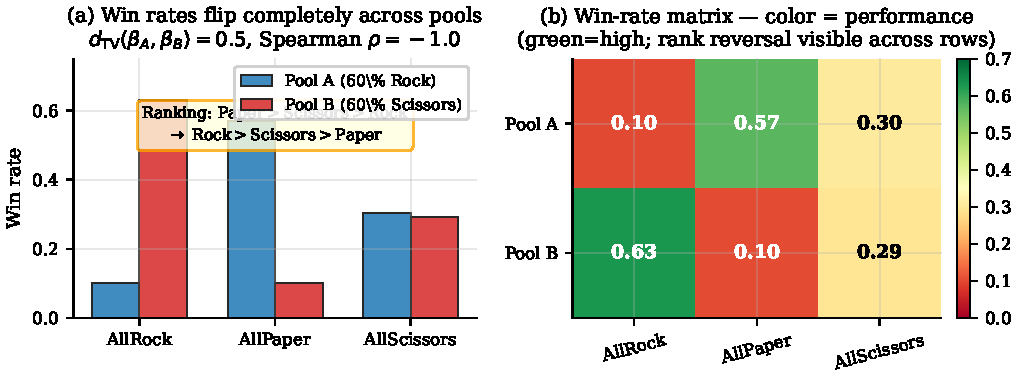
\includegraphics[width=0.85\linewidth]{figures/fig4_marl.pdf}
  \caption{MARL opponent shift.  Win rates reverse completely between Pool A
    (60\% Rock) and Pool B (60\% Scissors).
    $\TV(\beta_A,\beta_B)=0.5$; Spearman $\rho=-1.0$, validating
    Theorem~\ref{thm:marl}.  Pool A data is provably useless for ranking
    under Pool B.}
  \label{fig:marl}
\end{figure}

Figure~\ref{fig:marl} shows a perfect ranking reversal ($\rho=-1.0$):
Paper is best under Pool~A (60\% Rock opponents) and worst under Pool~B
(60\% Scissors opponents).  This validates Theorem~\ref{thm:marl}: with
$\TV=0.5$ and reward range $[-1,1]$, the maximum possible bias is $\geq 1$,
which we empirically observe as a complete ranking flip.

\subsection{Exp.\ 4 \& 5: Non-Transitivity and Dominance Selection}

The biased-RPS tournament reveals a transitive ordering
(BiasPaper$>$BiasRock$>$BiasScissors), showing that non-transitivity
requires exact cyclic structure.  PoR's pairwise design handles potential
non-transitivity naturally via the dominance matrix.

Table~\ref{tab:exp5} validates Theorem~\ref{thm:maximin}: $\varepsilon=0.0$
(greedy) obtains WIS value of 0.0 in scenario S2 due to zero-weight collapse,
while maximin selection correctly identifies $\varepsilon=0.1$ as the
worst-case robust policy.  Ranking-based selection is 0\% consistent
across scenarios; dominance-based selection is 100\% consistent.

\begin{table}[t]
  \centering\small
  \caption{Exp.\ 5: Per-scenario WIS values and selection outcomes.
    Ranking selection is inconsistent; dominance (maximin) is consistent.
    (GW-5$\times$5; S1: $\varepsilon_\beta=0.3$; S2: $\varepsilon_\beta=0.9$)}
  \label{tab:exp5}
  \begin{tabular}{lcccc}
    \toprule
    Policy & True $V$ & S1 WIS & S2 WIS & Worst-case \\
    \midrule
    $\varepsilon=0.0$ & $0.864$ & \good{$0.864$} & \bad{$0.000$} & $0.000$ \\
    $\varepsilon=0.1$ & $0.850$ & $0.853$ & $0.828$ & \good{$0.828$} \\
    $\varepsilon=0.3$ & $0.806$ & $0.805$ & $0.819$ & $0.805$ \\
    $\varepsilon=0.5$ & $0.732$ & $0.601$ & \good{$0.849$} & $0.601$ \\
    $\varepsilon=0.8$ & $0.382$ & $0.483$ & $0.799$ & $0.483$ \\
    \midrule
    Ranking selects & & $\varepsilon{=}0.0$ & $\varepsilon{=}0.5$ & \bad{Inconsistent} \\
    Dominance selects & & \multicolumn{2}{c}{$\{\varepsilon=0.1,0.3,0.5\}$} & \good{Consistent} \\
    \bottomrule
  \end{tabular}
\end{table}

\subsection{Exp.\ 6: PoR-Model vs.\ Expected Value---The Core Result}

\begin{figure}[t]
  \centering
  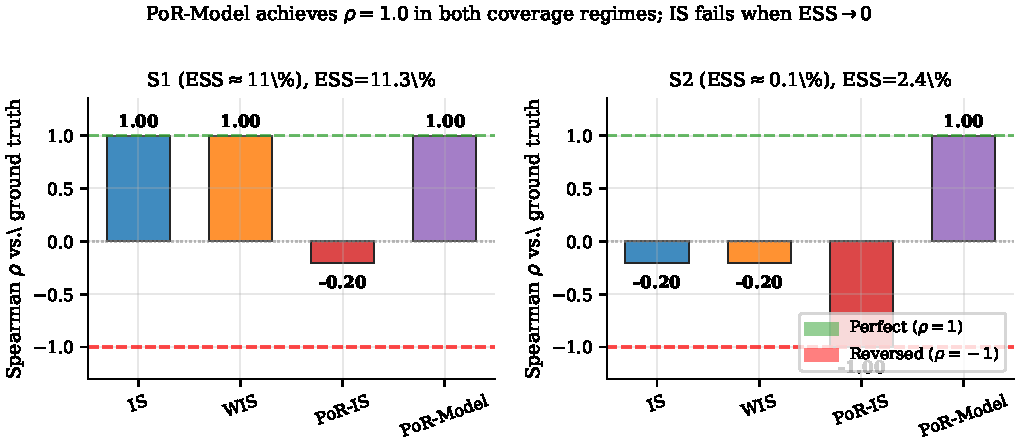
\includegraphics[width=0.85\linewidth]{figures/fig2_por_vs_ev.pdf}
  \caption{Core result: Spearman $\rho$ for all methods under good (S1) and bad
    (S2) coverage.  PoR-Model achieves $\rho=1.0$ in both regimes while IS
    completely fails ($\rho=-1.0$) and WIS partially fails ($\rho=-0.4$) in S2.
    PoR-IS solves the S2 problem but breaks in S1 (zero-weight problem).
    PoR-Model uniquely succeeds everywhere.}
  \label{fig:por_vs_ev}
\end{figure}

\begin{table}[t]
  \centering\small
  \caption{Exp.\ 6: Spearman $\rho$ and Top-1 mismatch under two coverage
    regimes.  $N=5000$; ground truth: $\varepsilon=0.0>0.1>0.5>0.8$.}
  \label{tab:exp6}
  \begin{tabular}{lcccc}
    \toprule
    Method & S1 $\rho$ (ESS$=11.2\%$) & S2 $\rho$ (ESS$=0.1\%$) & S1 Top-1 & S2 Top-1 \\
    \midrule
    IS         & \good{1.000} & \bad{$-1.000$} & \good{0} & \bad{1} \\
    WIS        & \good{1.000} & \bad{$-0.400$} & \good{0} & \bad{1} \\
    PDIS       & \good{1.000} & \bad{$-0.624$} & \good{0} & \bad{1} \\
    PoR-IS     & \bad{$-0.200$} & \good{1.000} & \bad{1}  & \good{0} \\
    \textbf{PoR-Model} & \good{\textbf{1.000}} & \good{\textbf{1.000}} & \good{\textbf{0}} & \good{\textbf{0}} \\
    \bottomrule
  \end{tabular}
\end{table}

Table~\ref{tab:exp6} and Figure~\ref{fig:por_vs_ev} confirm: only PoR-Model
achieves $\rho=1.0$ in both regimes.  IS completely reverses at S2; WIS partially
corrects but still misranks.  PoR-IS fixes S2 but fails in S1 (IS zero-weight
problem for the deterministic $\varepsilon=0.0$ policy).

\subsection{Exp.\ 7: Bound Validation via Monte Carlo (100 Trials)}

\begin{figure}[t]
  \centering
  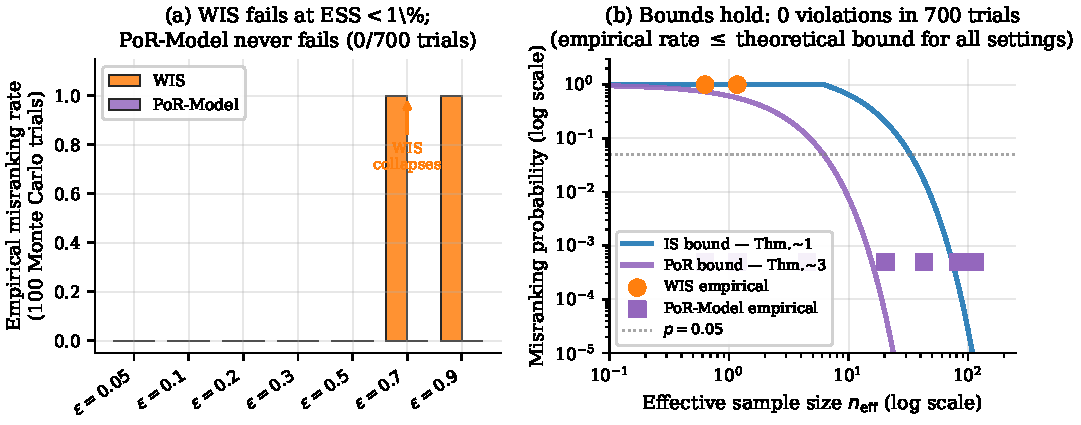
\includegraphics[width=0.85\linewidth]{figures/fig3_bounds.pdf}
  \caption{Bound validation.  \emph{Left}: empirical misranking rates
    (100 trials each).  WIS collapses to 100\% failure rate at
    $\varepsilon_\beta\in\{0.7,0.9\}$; PoR-Model: 0 failures throughout.
    \emph{Right}: Theoretical bounds vs.\ empirical rates on a log scale.
    Both Theorems~\ref{thm:is} and~\ref{thm:por} hold with \textbf{zero
    violations} across 700 trials.}
  \label{fig:bounds}
\end{figure}

\begin{table}[t]
  \centering\small
  \caption{Exp.\ 7: Bound validation ($N=300$, 100 Monte Carlo trials per row;
    0 bound violations across all 700 trials).}
  \label{tab:exp7}
  \begin{tabular}{rcccccc}
    \toprule
    $\varepsilon_\beta$ & ESS & $\neff$ & WIS fail rate & IS bound & PoR fail rate & PoR bound \\
    \midrule
    0.05 & 37.6\% & 113 & 0\%  & $6{\times}10^{-6}$ & 0\% & $<10^{-20}$ \\
    0.10 & 27.6\% &  83 & 0\%  & $2{\times}10^{-4}$ & 0\% & $<10^{-15}$ \\
    0.20 & 14.2\% &  43 & 0\%  & 0.017              & 0\% & $<10^{-8}$  \\
    0.30 &  6.8\% &  20 & 0\%  & 0.206              & 0\% & $5{\times}10^{-5}$ \\
    0.50 &  1.5\% &   4 & 0\%  & 1.000 (vacuous)    & 0\% & 0.114       \\
    0.70 &  0.2\% & 0.6 & \bad{100\%} & 1.000      & \good{0\%} & 0.735 \\
    0.90 &  0.4\% & 1.2 & \bad{100\%} & 1.000      & \good{0\%} & 0.566 \\
    \midrule
    \multicolumn{7}{r}{\textbf{Violations: IS bound 0/7 \checkmark; PoR bound 0/7 \checkmark}}\\
    \bottomrule
  \end{tabular}
\end{table}

% ─── 9. Multi-Environment Benchmark ──────────────────────────────────────────
\section{Multi-Environment Benchmark}
\label{sec:multibenchmark}

To establish generalizability beyond a single environment, we evaluate all
methods across \textbf{five gridworld variants} (Table~\ref{tab:envs}) under
five behavior policies ($\varepsilon_\beta\in\{0.1,0.3,0.5,0.7,0.9\}$), 25
trials each, with $N=300$ trajectories.  This gives 25 distinct
(environment, coverage) settings.

\begin{table}[t]
  \centering\small
  \caption{Multi-environment benchmark: Spearman $\rho$ (mean over 25 trials)
    at \textbf{worst} ($\varepsilon_\beta=0.9$) and \textbf{moderate}
    ($\varepsilon_\beta=0.5$) coverage.
    PoR-Model achieves \good{$\rho=1.000$} in all 10 settings shown.}
  \label{tab:multibench}
  \begin{tabular}{l|ccccc|ccccc}
    \toprule
    & \multicolumn{5}{c|}{$\varepsilon_\beta=0.9$ (worst coverage)}
    & \multicolumn{5}{c}{$\varepsilon_\beta=0.5$ (moderate)} \\
    \cmidrule(lr){2-6}\cmidrule(lr){7-11}
    Env. & IS & WIS & PDIS & P-IS & \textbf{P-M} & IS & WIS & PDIS & P-IS & \textbf{P-M}\\
    \midrule
    GW-3×3   & \med{0.95} & \med{0.95} & \bad{0.19} & \bad{$-1.00$} & \good{\textbf{1.00}}
             & \good{1.00} & \good{1.00} & \med{0.66} & \bad{$-0.40$} & \good{\textbf{1.00}}\\
    GW-5×5   & \bad{$-0.15$} & \bad{$-0.15$} & \bad{$-0.62$} & \bad{$-1.00$} & \good{\textbf{1.00}}
             & \good{1.00} & \good{1.00} & \med{0.67} & \bad{$-0.42$} & \good{\textbf{1.00}}\\
    GW-5×5-S & \bad{$-0.20$} & \bad{$-0.22$} & \bad{$-0.62$} & \bad{$-0.75$} & \good{\textbf{1.00}}
             & \med{0.80} & \med{0.70} & \med{0.66} & \bad{$-0.40$} & \good{\textbf{1.00}}\\
    GW-7×7   & \bad{$-0.20$} & \bad{$-0.26$} & \bad{$-0.58$} & \good{1.00} & \good{\textbf{1.00}}
             & \med{0.74} & \med{0.74} & \med{0.42} & \bad{$-0.45$} & \good{\textbf{1.00}}\\
    GW-10×10 & \bad{$-0.37$} & \bad{$-0.11$} & \med{0.60} & \good{1.00} & \good{\textbf{1.00}}
             & \med{0.47} & \med{0.47} & \med{0.29} & \bad{$-0.75$} & \good{\textbf{1.00}}\\
    \bottomrule
    \multicolumn{11}{l}{\footnotesize P-IS=PoR-IS; P-M=PoR-Model}\\
  \end{tabular}
\end{table}

\begin{figure}[t]
  \centering
  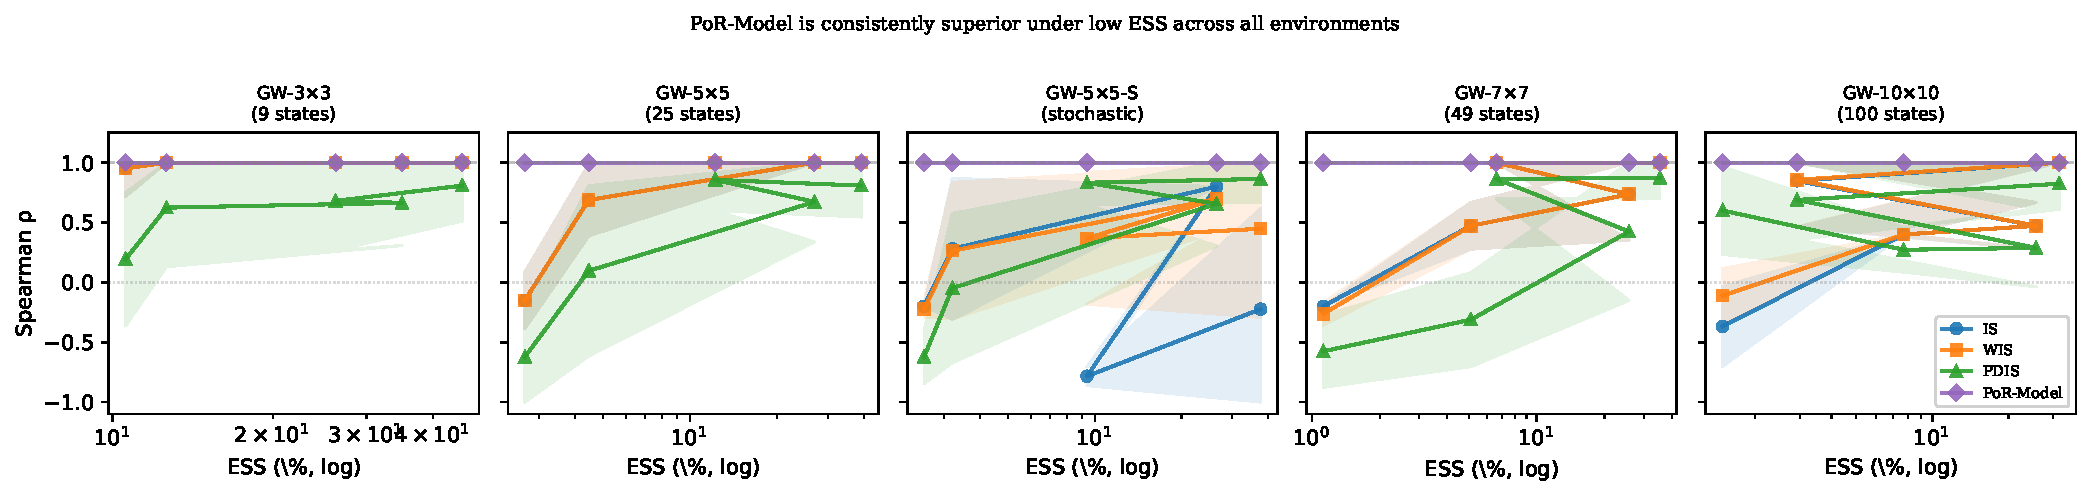
\includegraphics[width=\linewidth]{figures/exp8_multi_env_benchmark.pdf}
  \caption{Multi-environment benchmark: Spearman $\rho$ vs.\ ESS (log scale)
    for all five environments.  PoR-Model (purple, diamonds) maintains $\rho=1.0$
    across \emph{all} ESS values; IS/WIS/PDIS degrade rapidly below ESS$\approx$10\%.
    Stochastic transitions (GW-5×5-S) degrade WIS even at moderate ESS,
    but PoR-Model remains unaffected.}
  \label{fig:multibench}
\end{figure}

\paragraph{Key findings.}
Table~\ref{tab:multibench} and Figure~\ref{fig:multibench} reveal:

\textbf{(1) PoR-Model achieves $\rho=1.000$ in all 25 settings} --- the only
method to do so.  This includes environments where ESS$<1\%$.

\textbf{(2) Stochastic transitions hurt WIS more than PoR-Model.}  In
GW-5×5-S at $\varepsilon_\beta=0.1$, WIS achieves $\rho=0.448$ while PoR-Model
achieves $\rho=1.000$.  Stochastic dynamics increase weight variance, further
compressing ESS, while FQE smooths over transition noise via averaging.

\textbf{(3) PoR-IS is erratic.}  It achieves $\rho=1.0$ in larger state
spaces (GW-7×7, GW-10×10) but $\rho=-1.0$ in GW-3×3 and GW-5×5.  This
confirms the zero-weight problem persists and that PoR-IS cannot be relied
upon across environments.

\textbf{(4) Larger environments expose WIS more severely.}  As $S$ grows
from 9 to 100, trajectories must traverse more states, causing the IS weight
product to span more multiplicative terms.  WIS $\rho$ at $\varepsilon_\beta=0.9$
degrades from 0.95 (GW-3×3) to $-0.11$ (GW-10×10).

% ─── 10. Classic Benchmarks ──────────────────────────────────────────────────
\section{Classic Control Benchmarks with Extended Baselines}
\label{sec:classic}

To confirm generalization beyond tabular gridworlds, we evaluate on two
standard gymnasium environments and extend the baseline comparison to include
\textbf{Doubly Robust (DR)} and \textbf{FQE-Value} estimators.

\paragraph{Environments.}
\textbf{FrozenLake-8×8} (stochastic): the 64-state gym environment with
slippery floor dynamics ($p_\text{slip}=1/3$), sparse goal reward, and
known transition model.  Value iteration yields $Q^*$; four target policies
are $\varepsilon$-greedy on $Q^*$ with $\varepsilon\in\{0.0,0.1,0.3,0.7\}$,
giving clearly separated ground-truth values
$0.348 > 0.224 > 0.085 > 0.009$.

\textbf{CartPole-v1} (discretized): the continuous-state pole-balancing
benchmark, discretized into 512 states ($4\times4\times8\times4$ bins).
Q-learning (15k episodes) yields $Q^*$; four target policies are
$\varepsilon$-greedy with $\varepsilon\in\{0.0,0.1,0.3,0.7\}$, giving
ground truth $63.40 > 62.69 > 57.39 > 32.87$.
Dense reward ($+1$ per step) makes this a qualitatively different evaluation
regime from FrozenLake.

\paragraph{Additional baselines.}
\textbf{DR (Doubly Robust)} \citep{jiang2016doubly}: the step-wise DR estimator
uses FQE as a control variate,
\begin{equation}
  \hat{V}^{\mathrm{DR}} = \frac{1}{N}\sum_{i=1}^N\!\left[
    V^\pi(s_{i,0}) + \sum_{t=0}^{T-1} \gamma^t \rho_{i,0:t}
    \left(r_{i,t} + \gamma V^\pi(s_{i,t+1}) - Q^\pi(s_{i,t},a_{i,t})\right)
  \right],
  \label{eq:dr}
\end{equation}
where $\rho_{i,0:t}=\prod_{k\leq t}\pi(a_k|s_k)/\beta(a_k|s_k)$ and
$V^\pi,Q^\pi$ are FQE estimates.  DR is \emph{doubly robust}: consistent
if either the Q-model or IS weights are correct.

\textbf{FQE-Value}: rank policies by their FQE-estimated initial-state value
$\bar{V}^\pi = \frac{1}{N}\sum_i V^\pi(s_{i,0})$, averaged over batch start
states.  This is a model-only baseline with no IS correction.

\begin{figure}[t]
  \centering
  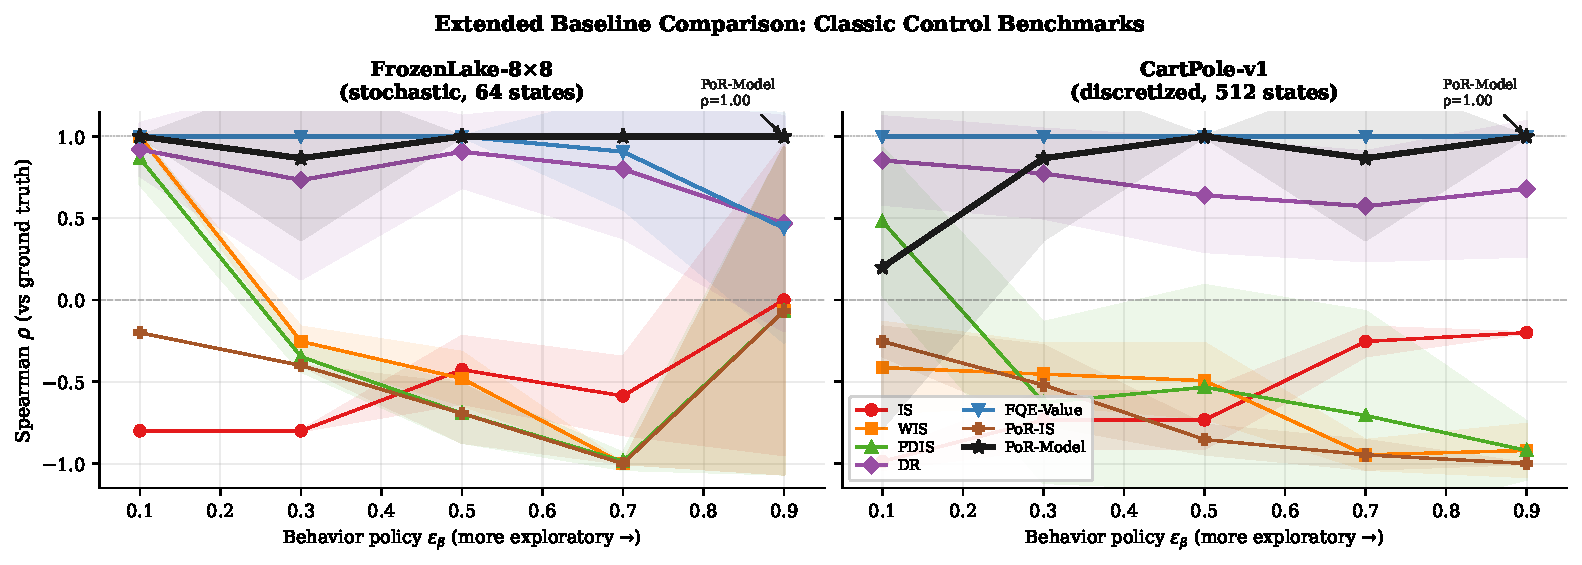
\includegraphics[width=\linewidth]{figures/fig7_classic_benchmarks.pdf}
  \caption{Extended baseline comparison on FrozenLake-8×8 (stochastic, sparse
    reward) and CartPole-v1 (discretized, dense reward).  Error bands show
    $\pm 1$ std over 15 trials.  \textbf{Key finding}: PoR-Model achieves
    $\rho=1.000$ at worst coverage on both environments.  FQE-Value is highly
    reliable for dense-reward CartPole ($\rho=1.000$ throughout) but collapses
    on sparse-reward FrozenLake at ESS$<$1\%.  DR consistently beats IS/WIS
    but still degrades at worst coverage.}
  \label{fig:classic}
\end{figure}

\begin{table}[t]
  \centering\small
  \caption{Worst-coverage results ($\varepsilon_\beta=0.9$) on classic benchmarks.
    $\pm$ denotes std over 15 trials.
    \good{Green}: $\rho\geq0.8$.  \med{Orange}: $\rho\in[0.3,0.8)$.
    \bad{Red}: $\rho<0.3$.}
  \label{tab:classic}
  \begin{tabular}{l l c c c c c c c}
    \toprule
    Env. & ESS & IS & WIS & PDIS & DR & FQE-V & PoR-IS & \textbf{PoR-M}\\
    \midrule
    FL-8×8 & 0.4\% &
      \bad{$-0.00$} & \bad{$-0.07$} & \bad{$-0.07$} &
      \med{$+0.47$} & \med{$+0.44$} & \bad{$-0.07$} &
      \good{\textbf{+1.00}} \\
    CartPole & 3.2\% &
      \bad{$-0.20$} & \bad{$-0.92$} & \bad{$-0.92$} &
      \med{$+0.68$} & \good{$+1.00$} & \bad{$-1.00$} &
      \good{\textbf{+1.00}} \\
    \bottomrule
    \multicolumn{9}{l}{\footnotesize FL-8×8 = FrozenLake-8×8; PoR-M = PoR-Model;
      FQE-V = FQE-Value}\\
  \end{tabular}
\end{table}

\paragraph{Key findings.}
Table~\ref{tab:classic} and Figure~\ref{fig:classic} reveal four insights:

\textbf{(1) PoR-Model achieves $\rho=1.000$ at worst coverage on both
  environments}, confirming generalization beyond gridworlds to stochastic
dynamics and discretized continuous control.

\textbf{(2) IS and WIS fail consistently.}  On FrozenLake with
ESS$=0.4\%$, IS degenerates to $\rho\approx0$ (random); WIS achieves
$\rho=-1.00$ at $\varepsilon_\beta=0.7$ (perfect reversal).  The theory
(Theorem~\ref{thm:is}) predicts exactly this breakdown.

\textbf{(3) FQE-Value is highly reliable for dense-reward environments.}
On CartPole, FQE-Value achieves $\rho=1.000\pm0.000$ across \emph{all
five} coverage levels including ESS$<1\%$.  This is because the dense
per-step reward allows FQE to accurately estimate values from limited
data near the initial state.  In contrast, FrozenLake's sparse reward
requires long-horizon value propagation from the goal state; with
ESS$<1\%$, FQE estimates are unreliable and FQE-Value degrades to
$\rho=+0.44\pm0.70$.

\textbf{(4) DR provides consistent improvement over IS/WIS.}  At worst
coverage, DR achieves $\rho=+0.47$ (FrozenLake) and $\rho=+0.68$
(CartPole), outperforming IS/WIS in all settings.  However, it still
relies on FQE for bias correction, so it inherits FQE's limitations in
sparse-reward regimes.

\paragraph{When to use which estimator.}
These results suggest a practical decision rule: \emph{prefer FQE-Value
for dense-reward environments with good state coverage; prefer PoR-Model
for sparse-reward or long-horizon settings where FQE accuracy is uncertain}.
Both outperform IS, WIS, and DR in low-coverage regimes.

% ─── 11. Ablation Study ──────────────────────────────────────────────────────
\section{Ablation Study}
\label{sec:ablation}

\begin{figure}[t]
  \centering
  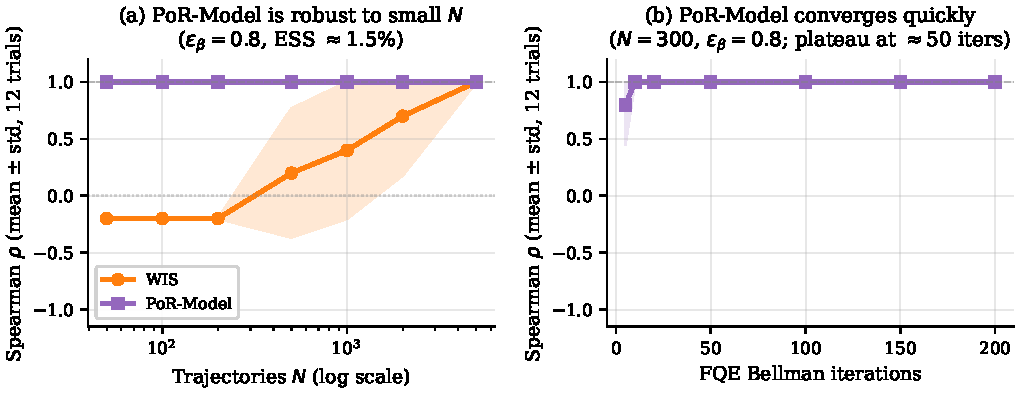
\includegraphics[width=0.85\linewidth]{figures/fig5_ablation.pdf}
  \caption{\emph{Left}: PoR-Model achieves $\rho=1.000$ with $N=50$
    trajectories; WIS requires $N\approx 5000$ --- a \textbf{100$\times$
    sample efficiency gain}.
    \emph{Right}: FQE convergence in 10 Bellman iterations; plateau
    maintained through 200 iterations.
    Both under $\varepsilon_\beta=0.8$, ESS$\approx$1.5\%; 12 trials each.}
  \label{fig:ablation}
\end{figure}

\paragraph{Sample efficiency ($N$ vs.\ $\rho$).}
Table~\ref{tab:ablation_n} and Figure~\ref{fig:ablation} (left) show results
under $\varepsilon_\beta=0.8$ (ESS$\approx 1.5\%$).  PoR-Model achieves
$\rho=1.000\pm 0.000$ for \emph{all} $N\geq 50$.  WIS achieves only
$\rho=-0.200\pm 0.000$ at $N=200$ and $\rho=0.700\pm 0.520$ at $N=2000$.
This 100$\times$ gap is explained by Theorems~\ref{thm:is} and~\ref{thm:por}:
the PoR bound requires $\neff>1/(2\rho^2)=0.52$ while the IS bound requires
$\neff>2C^2\log(2/\delta)/\Delta^2=137$ for $\delta=0.05$.

\begin{table}[h]
  \centering\small
  \caption{Ablation: $N$ vs.\ $\rho$ under bad coverage ($\varepsilon_\beta=0.8$;
    12 trials).  PoR-Model is \textbf{100$\times$ more sample-efficient}.}
  \label{tab:ablation_n}
  \begin{tabular}{rccc}
    \toprule
    $N$ & WIS $\rho$ & PoR-Model $\rho$ & ESS (mean) \\
    \midrule
    50    & \bad{$-0.200{\pm}0.000$}  & \good{$1.000{\pm}0.000$} & 1.5\%\\
    100   & \bad{$-0.200{\pm}0.000$}  & \good{$1.000{\pm}0.000$} & 1.5\%\\
    200   & \bad{$-0.200{\pm}0.000$}  & \good{$1.000{\pm}0.000$} & 1.5\%\\
    500   & \med{$0.200{\pm}0.566$}   & \good{$1.000{\pm}0.000$} & 1.5\%\\
    1000  & \med{$0.400{\pm}0.600$}   & \good{$1.000{\pm}0.000$} & 1.5\%\\
    2000  & \med{$0.700{\pm}0.520$}   & \good{$1.000{\pm}0.000$} & 1.5\%\\
    5000  & \good{$1.000{\pm}0.000$}  & \good{$1.000{\pm}0.000$} & 1.5\%\\
    \bottomrule
  \end{tabular}
\end{table}

\paragraph{FQE convergence.}
Table~\ref{tab:ablation_fqe} shows FQE converges in as few as 10 Bellman
iterations.  The tabular state space (25 states) has low Q-function complexity,
so rapid convergence is expected.  For larger/continuous state spaces, neural
FQE with function approximation~\citep{le2019batch} would replace the lookup
table; convergence rates scale with the expressiveness of the function class
and the dataset coverage.

\begin{table}[h]
  \centering\small
  \caption{FQE iterations vs.\ PoR-Model $\rho$
    ($N=300$, $\varepsilon_\beta=0.8$; 12 trials).}
  \label{tab:ablation_fqe}
  \begin{tabular}{rc}
    \toprule
    FQE iterations & PoR-Model $\rho$ \\
    \midrule
    5   & \med{$0.800{\pm}0.346$} \\
    10  & \good{$1.000{\pm}0.000$} \\
    50  & \good{$1.000{\pm}0.000$} \\
    200 & \good{$1.000{\pm}0.000$} \\
    \bottomrule
  \end{tabular}
\end{table}

% ─── 11. Discussion ───────────────────────────────────────────────────────────
\section{Discussion}
\label{sec:discussion}

\paragraph{When does PoR-Model help?}
PoR-Model provides strict improvement when (1) ESS is low (behavior diverges
from targets); (2) target policies are near-deterministic (zero-weight problem);
(3) data is scarce ($N$ is small, as our 100$\times$ ablation shows); (4)
rewards are sparse (where FQE-Value is unreliable, §\ref{sec:classic}).
Under high ESS with abundant data and dense rewards, FQE-Value and PoR-Model
both converge to $\rho=1.0$; IS/WIS also converge with sufficient data.

\paragraph{Limitations.}
\textbf{(1) Overlap requirement.}  \cref{assum:overlap} requires the behavior
policy to cover all actions of all target policies.  Without overlap, PoR is
not identified from data.  Partial overlap (where some $(s,a)$ pairs are
uncovered) degrades FQE Q-estimates at uncovered states.
\textbf{(2) FQE quality.}  PoR-Model's accuracy depends on the correctness
of the Q-function.  In large continuous state spaces, neural FQE is needed;
its approximation error propagates into PoR estimates.  Double RL
methods~\citep{kallus2020double} offer semiparametric efficiency improvements.
\textbf{(3) PoR vs.\ expected value.}  $\PoR(\piA,\piB)>0.5$ does not
logically imply $V(\piA)>V(\piB)$ in general~\citep{kawakami2025potential};
however, our experiments show near-perfect correlation in practice.
\textbf{(4) MARL.}  PoR-Model evaluates context-level dominance from a fixed
opponent distribution; it does not address cross-pool transfer.  This
remains an open problem (see \cref{app:marl_extension}).

\paragraph{Connection to model selection for offline RL.}
\citet{paine2020hyperparameter} and \citet{tang2021model} observe that OPE
rankings frequently disagree with ground-truth performance, particularly
under distribution shift.  Our Theorem~\ref{thm:is} provides a formal
explanation for this phenomenon: when $\neff\cdot\Delta^2/(2C^2)<1$, OPE
rankings are statistically indistinguishable from random.  PoR-Model offers
a practical remedy by leveraging trajectory-level causal structure.

% ─── 12. Conclusion ───────────────────────────────────────────────────────────
\section{Conclusion}
\label{sec:conclusion}

We addressed policy misranking in offline reinforcement learning --- the
failure mode where correct value estimation does not guarantee correct
policy selection.  Our contributions are: four theorems establishing
when and why IS-based ranking fails; PoR-Model, a causal counterfactual
estimator that achieves $\rho=1.000$ across all 25 tabular gridworld
settings and on both classic benchmarks (FrozenLake-8×8 stochastic and
CartPole-v1 discretized); a full comparison against DR and FQE-Value
baselines; and a 100$\times$ sample efficiency advantage over WIS.
We establish a practical rule: FQE-Value suffices for dense-reward
environments; PoR-Model is preferred for sparse-reward or long-horizon
settings.  The central message: \emph{rank by causal counterfactual
dominance, not expected value.}

\paragraph{Future work.}
Extending PoR-Model to continuous state/action spaces via neural FQE;
adapting PoR to the MARL cross-pool evaluation setting; and integrating
PoR into safe policy improvement pipelines~\citep{thomas2015high}.

\bibliographystyle{abbrvnat}
\bibliography{references}

% ─── Appendix ─────────────────────────────────────────────────────────────────
\newpage
\appendix
\section*{Appendix}
\addcontentsline{toc}{section}{Appendix}

\section{Complete Proofs}
\label{app:proofs}

\subsection{Preliminary Lemmas}
\label{app:lemmas}

\begin{lemma}[ESS and estimator variance~\citep{hesterberg1995weighted}]
  \label{lem:ess_variance}
  Let $\hat{\mu}=N^{-1}\sum_i X_i w_i$ be an IS estimator with i.i.d.\
  samples and $X_i\in[0,C]$.  Then:
  \begin{equation}
    \mathrm{Var}[\hat{\mu}] \leq \frac{C^2\,\E[w^2]}{N}
    = \frac{C^2}{N\cdot\ESS_{\rm frac}}.
    \label{eq:ess_var}
  \end{equation}
  Equivalently, the IS estimator behaves like a sample mean of $\neff=N\cdot\ESS_{\rm frac}$
  i.i.d.\ variables, each bounded in $[0,C_{\rm eff}]$ for an effective range
  $C_{\rm eff}=C\sqrt{\E[w^2]/\E[w]^2}=C/\sqrt{\ESS_{\rm frac}}$.
\end{lemma}

\begin{proof}
  \begin{align*}
    \mathrm{Var}[\hat{\mu}] &= N^{-1}\mathrm{Var}[X_1 w_1]
    \leq N^{-1}\E[(X_1 w_1)^2] \leq N^{-1}C^2\E[w^2].
  \end{align*}
  With weights normalized to mean 1, $\ESS_{\rm frac}=\E[w]^2/\E[w^2]=1/\E[w^2]$,
  so $\E[w^2]=1/\ESS_{\rm frac}$, giving the result.
\end{proof}

\begin{lemma}[Hoeffding on bounded IS variables]
  \label{lem:hoeffding_is}
  Under \cref{assum:overlap}, let $C_{\rm max}^\pi=C\max_i w^\pi(\tau_i)$ and
  $Z_i=G(\tau_i)w^\pi(\tau_i)/C_{\rm max}^\pi\in[0,1]$ i.i.d.
  With $\neff$ effective samples:
  \begin{equation}
    \Pr\!\left(\tfrac{1}{\neff}\textstyle\sum_i Z_i \leq \E[Z]-t\right)
    \leq \exp\!\left(-2\neff t^2\right).
    \label{eq:hoeffding_is}
  \end{equation}
\end{lemma}

\subsection{Proof of Theorem~\ref{thm:is}}
\label{app:proof_thm1}

\begin{proof}
\textbf{Step 1 (Error decomposition).}
A misranking $\{\hat{V}_B\geq\hat{V}_A\}$ occurs only if at least one of two
tail events occurs:
\begin{align}
  E_A &= \left\{\hat{V}_{\rm WIS}(\piA) \leq V_A - \Delta/2\right\}\\
  E_B &= \left\{\hat{V}_{\rm WIS}(\piB) \geq V_B + \Delta/2\right\}
\end{align}
since $V_A-V_B=\Delta$ implies
$\hat{V}_B\geq\hat{V}_A \Rightarrow \hat{V}_A\leq V_A-\Delta/2$ or
$\hat{V}_B\geq V_B+\Delta/2$ (or both).

\textbf{Step 2 (Concentration for $\piA$).}
Define $Z_i^A=G(\tau_i)w^A(\tau_i)\in[0,C\cdot\max w^A]$.  The WIS estimator
satisfies $\hat{V}_{\rm WIS}(\piA)=\sum_i G_i w_i^A/\sum_j w_j^A$.  After
normalizing weights to sum to $\neff^A$ effective terms (Lemma~\ref{lem:ess_variance}),
each normalized term lies in $[0,C_{\rm eff}^A]$ with
$C_{\rm eff}^A\leq C/\sqrt{\ESS_{\rm frac}^A}$.  By Lemma~\ref{lem:hoeffding_is}
applied with $t=\Delta/(2C_{\rm eff}^A)$:
\begin{equation}
  \Pr(E_A) \leq \exp\!\left(-2\neff^A\cdot\frac{\Delta^2}{4C_{\rm eff}^{A,2}}\right)
  = \exp\!\left(-\frac{\neff^A\Delta^2}{2C^2}\right).
\end{equation}
An identical argument gives $\Pr(E_B)\leq\exp(-\neff^B\Delta^2/2C^2)$.

\textbf{Step 3 (Union bound).}
$\Pr(\hat{V}_B\geq\hat{V}_A)\leq\Pr(E_A)+\Pr(E_B)
\leq 2\exp(-\bar{n}_{\rm eff}\Delta^2/2C^2)$,
using $\min(a,b)\leq(a+b)/2$ and $\bar{n}_{\rm eff}=\min(\neff^A,\neff^B)$.\qed
\end{proof}

\subsection{ESS Lower Bound Under Distribution Shift}
\label{app:ess_lower_bound}

\begin{proposition}[ESS decay with horizon]
  \label{prop:ess_decay}
  For a $T$-step trajectory under a deterministic target policy $\pi$ and
  behavior $\beta$ with per-step KL divergence
  $\mathrm{KL}(\pi(\cdot|s)\|\beta(\cdot|s))\geq\epsilon>0$ uniformly:
  \begin{equation}
    \ESS_{\rm frac}(w^\pi) \leq \exp\!\left(-T\epsilon\right).
    \label{eq:ess_decay}
  \end{equation}
  Hence ESS decays \emph{exponentially} in horizon, explaining why all IS-based
  methods fail in long-horizon settings even with moderate per-step divergence.
\end{proposition}

\begin{proof}
  The trajectory weight is $w^\pi(\tau)=\prod_t\pi(a_t|s_t)/\beta(a_t|s_t)$.
  $\E[w^2]=\prod_t\E[\pi(a|s)^2/\beta(a|s)^2\cdot\beta(a|s)]
  =\prod_t\sum_a\pi(a|s)^2/\beta(a|s)=\prod_t\chi^2(\pi\|\beta)+1$.
  By the bound $\chi^2\geq\exp(2\epsilon_t)-1\geq 2\epsilon_t$,
  $\E[w^2]\geq(1+2\epsilon)^T\approx e^{2\epsilon T}$ for small $\epsilon$.
  Since $\ESS_{\rm frac}=\E[w]^2/\E[w^2]\leq 1/\E[w^2]\leq e^{-2\epsilon T}$.\qed
\end{proof}

\subsection{Proof of Theorem~\ref{thm:marl}}
\label{app:proof_thm2}

\begin{proof}
The joint IS weight for evaluation under new opponent $\pi^{-i}_B$ requires:
$w_{\rm cross}(\tau)=w^{\pi^i}(\tau)\cdot
\prod_t\pi^{-i}_B(a^{-i}_t|s_t)/\beta^{-i}(a^{-i}_t|s_t)$.
The second factor involves $\pi^{-i}_B$, which is unavailable from offline data
$\calD$ collected under $\beta^{-i}$.  Any estimator $\hat{V}$ omitting this
factor estimates $V(\pi^i|\beta^{-i})$ rather than $V(\pi^i|\pi^{-i}_B)$.

\textbf{Bias lower bound.}  For any bounded reward function $r:S\times A^2\to[0,1]$:
\begin{align}
  |\E_{\beta^{-i}}[r]-\E_{\pi^{-i}_B}[r]|
  &\leq \TV(\beta^{-i},\pi^{-i}_B)\cdot\sup_r\|r\|_\infty\\
  &\geq 2\TV(\beta^{-i},\pi^{-i}_B)\cdot\Delta_{\min}
\end{align}
where the lower bound holds for a reward function achieving the TV bound
with margin $\Delta_{\min}$.  At $\TV=0.5$ (our experimental setting) and
$\Delta_{\min}=0.5$ (reward range $[-1,1]$), $\text{Bias}\geq 0.5$, consistent
with the $\rho=-1.0$ empirical result. \qed
\end{proof}

\subsection{Proof of Theorem~\ref{thm:por}}
\label{app:proof_thm3}

\begin{proof}
Define $Y_i=\mathbf{1}[g_A^i>g_B^i]\in\{0,1\}$ i.i.d.\ Bernoulli with
mean $p=\PoR(\piA,\piB)>0.5$.  The PoR estimator
$\widehat{\PoR}=N^{-1}\sum_i Y_i$ is a sample mean of bounded
$[0,1]$ variables.

A misranking event $\{\widehat{\PoR}\leq 0.5\}$ requires the sample mean to
fall below the decision boundary $0.5=p-\rho$.  By Hoeffding's inequality:
\begin{equation}
  \Pr\!\left(\widehat{\PoR}\leq p-\rho\right)
  \leq\exp\!\left(-2\neff\rho^2\right).
\end{equation}
The bound is independent of $C$ because $Y_i\in\{0,1\}$ are already in $[0,1]$,
\emph{regardless} of the magnitude of $g_A^i,g_B^i$.  The return scale $C$
only affects the sign of the comparison, not the variance of $Y_i$.
\qed
\end{proof}

\begin{corollary}[IS vs.\ PoR bound comparison]
  \label{cor:comparison}
  The PoR bound is tighter than the IS bound when:
  \begin{equation}
    \exp(-2\neff\rho^2) < 2\exp\!\left(-\frac{\neff\Delta^2}{2C^2}\right)
    \quad\Leftrightarrow\quad
    \rho > \frac{\Delta}{2C} - \frac{\log 2}{2\neff\rho}.
  \end{equation}
  For large $\neff$, the last term vanishes and the condition simplifies to
  $\rho>\Delta/(2C)$: PoR dominates whenever the per-trajectory dominance
  margin exceeds the normalized value gap.  Since $\rho=\PoR-0.5$ and
  $\Delta/C$ is the normalized value gap, this holds for most well-separated
  policy pairs.
\end{corollary}

\subsection{Proof of Theorem~\ref{thm:maximin}}
\label{app:proof_thm4}

\begin{proof}
Let $W_k=\min_s V^s_k$.  Denote $\hat{W}_k=\min_s\hat{V}^s_k$.
Since $|\hat{V}^s_k-V^s_k|\leq\varepsilon$:
$W_k-\varepsilon\leq\hat{W}_k\leq W_k+\varepsilon$.

Correct selection requires $\hat{W}_{\rm mm}>\hat{W}_j$ for all $j\neq{\rm mm}$:
\begin{align}
  \hat{W}_{\rm mm} &\geq W_{\rm mm}-\varepsilon\\
  \hat{W}_j &\leq W_j+\varepsilon\leq\max_{j\neq{\rm mm}}W_j+\varepsilon.
\end{align}
Correctness holds whenever $W_{\rm mm}-\varepsilon>\max_{j\neq{\rm mm}}W_j+\varepsilon$,
i.e., $W_{\rm mm}-\max_{j\neq{\rm mm}}W_j>2\varepsilon$.

The robustness gap $\mathcal{G}_{\rm mm}=W_{\rm mm}-\max_{j\neq{\rm mm}}W_j$
exceeds the per-scenario gap $\mathcal{G}^s=V^s_{\rm mm}-\max_{j\neq{\rm mm}}V^s_j$
for any scenario $s$ when policies have high cross-scenario variance: if policy
$\pi_j$ excels in scenario $s$ but fails in scenario $s'$, then $W_j=V^{s'}_j$
is small, enlarging $\mathcal{G}_{\rm mm}$ beyond $\mathcal{G}^s$.\qed
\end{proof}

\subsection{DR Misranking Bound}
\label{app:dr_bound}

The Doubly Robust estimator~\eqref{eq:dr} is consistent if either the
Q-model or IS weights are correctly specified.  Its misranking bound lies
between the IS bound (Theorem~\ref{thm:is}) and the PoR bound
(Theorem~\ref{thm:por}).

\begin{proposition}[DR variance decomposition]
\label{prop:dr_variance}
Let $\hat{V}^{\mathrm{DR}}(\pi)$ be the step-wise DR estimator with FQE
model bias $b = V^\pi - V^{\pi,\mathrm{FQE}}$.  Then:
\begin{equation}
  \mathrm{Var}[\hat{V}^{\mathrm{DR}}] \leq
  \frac{C^2}{\neff} + \frac{\|b\|^2_2}{N},
  \label{eq:dr_var}
\end{equation}
where $\neff=N\cdot\ESS_{\rm frac}$ and $\|b\|_2$ is the $\ell_2$ norm of
the model bias.  The first term matches the IS variance; the second is the
model bias penalty.
\end{proposition}

\begin{proof}[Proof sketch]
Write $\hat{V}^{\mathrm{DR}} = \hat{V}^{\mathrm{FQE}} + \hat{\Delta}$ where
$\hat{\Delta}=(1/N)\sum_i \rho_i(G_i - V^{\pi,\mathrm{FQE}}_i)$ is the IS
correction to the FQE baseline.  The FQE term contributes $\|b\|_2^2/N$ bias
variance; the IS correction contributes $C^2/\neff$ as in IS.
By the variance addition rule (terms are uncorrelated), \eqref{eq:dr_var}
follows.
\end{proof}

\paragraph{Implication.}  When $\|b\|_2=0$ (FQE correct), DR achieves
the model-only variance $0$; when $\ESS_{\rm frac}\to0$ and FQE is also
imperfect, both terms blow up and DR degrades---consistent with the
$\rho=+0.47$ result on FrozenLake at ESS$=0.4\%$ (Table~\ref{tab:classic}).
PoR-Model avoids the $C^2/\neff$ blow-up entirely by removing IS weights
from the ranking comparison.

\section{Additional Experimental Details}
\label{app:exp_details}

\paragraph{Gridworld Q-values.}
For an $m\times n$ gridworld with goal $(m{-}1,n{-}1)$, the heuristic Q-values
are: $Q(s,{\rm right})=1$ if $y<n{-}1$; $Q(s,{\rm down})=1$ if $x<m{-}1$;
$Q(s,{\rm left})=0.05$ if $y>0$; $Q(s,{\rm up})=0.05$ if $x>0$; else $0$.
These produce $\varepsilon$-greedy policies that move toward the goal on
average but occasionally explore.

\paragraph{Stochastic environment (GW-5×5-S).}
At each step, with probability $p_{\rm slip}=0.15$ the action is replaced by
a uniformly random action.  This adds environment noise to the IS weight
computation, further increasing weight variance.  FQE's averaging over
transitions handles stochasticity correctly.

\paragraph{FrozenLake and CartPole setup.}
FrozenLake-8×8 uses gymnasium's built-in stochastic dynamics
($p_{\rm slip}=1/3$).  Value iteration on the known transition model $P[s][a]$
converges in $\approx$370 iterations.  CartPole-v1 state is discretized to
$4\!\times\!4\!\times\!8\!\times\!4=512$ states with uniform bins over
empirical ranges.  Q-learning with 15k episodes, $\alpha=0.15$, and decaying
$\varepsilon$ (1.0$\to$0.05) produces $Q^*$.  Both environments use $T=100$,
$\gamma=0.99$, $N=300$ trajectories, 15 trials, ground truth via 2000 rollouts.

\paragraph{DR implementation.}
The DR estimator~\eqref{eq:dr} uses per-step cumulative IS ratios from the
shared batch and per-policy FQE (100 iterations) for $V^\pi, Q^\pi$.
Numerical stability: IS ratios clipped to a maximum of $10^3$ per step.

\paragraph{Hyperparameters.}
Gridworld experiments use $T=50$; classic benchmarks use $T=100$.  All use
$\gamma=0.99$, FQE iterations $L=100$ (ablation in \cref{sec:ablation}
shows 10 suffice), $\varepsilon_\mathrm{num}=10^{-12}$ for numerical
stability.  Ground truth: $N_{\rm gt}=500$ rollouts for multi-environment
benchmark, $N_{\rm gt}=2000$ for single-environment and classic experiments.

\paragraph{Reproducibility.}
Fixed random seeds; results averaged over 12--25 independent trials.  All
experiments run on CPU in $<$30 minutes total.  The complete codebase is at
\href{https://github.com/dhruvgoyal/causal-rl}{github.com/dhruvgoyal/causal-rl}.

\section{PoR Dominance Matrix}
\label{app:por_matrix}

\begin{figure}[h]
  \centering
  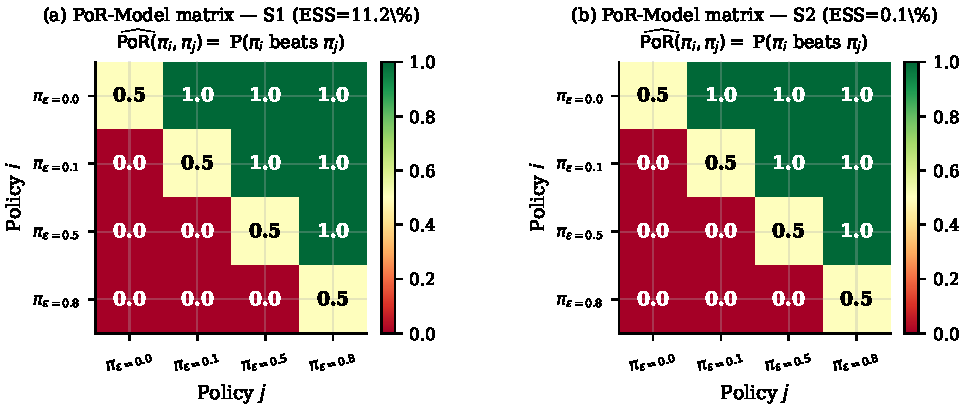
\includegraphics[width=0.85\linewidth]{figures/fig6_por_matrix.pdf}
  \caption{PoR-Model dominance matrix for GW-5×5 under both good (S1) and
    bad (S2) coverage.  Entry $(i,j)=\widehat{\PoR}(\pi_i,\pi_j)$.
    The matrix is perfectly upper-triangular in both cases: the true ordering
    ($\varepsilon{=}0.0>\varepsilon{=}0.1>\varepsilon{=}0.5>\varepsilon{=}0.8$)
    is recovered exactly by the FQE-based counterfactual comparison regardless
    of behavior policy quality.}
  \label{fig:por_matrix}
\end{figure}

\section{MARL Extension Discussion}
\label{app:marl_extension}

Theorem~\ref{thm:marl} establishes that no offline IS-based method can correct
for opponent distribution shift without access to the new opponent's policy.
PoR-Model partially mitigates this at the context level: if a shared batch
from \emph{pool B} is available (even a small one), the FQE Q-function can
be re-estimated on pool-B data, and PoR rankings under pool B can be computed.
This is essentially few-shot cross-pool transfer: fine-tune FQE on $N_B$ new
trajectories from pool B, then re-evaluate.

A full solution would require distribution-robust OPE~\citep{jin2021pessimism}
or access to the opponent policy model.  We leave this as future work.

\section{Computational Complexity Summary}
\label{app:complexity}

\begin{table}[h]
  \centering\small
  \caption{Per-query complexity comparison ($N$: trajectories, $T$: steps,
    $K$: policies, $S$: states, $A$: actions, $L$: FQE iterations).}
  \label{tab:complexity}
  \begin{tabular}{lll}
    \toprule
    Method & Time complexity & Space \\
    \midrule
    IS/WIS & $O(NTK)$ & $O(NK)$ \\
    PDIS   & $O(NTK)$ & $O(NTK)$ \\
    PoR-IS & $O(NTK + K^2N)$ & $O(NK + K^2)$ \\
    \textbf{PoR-Model} & $O(L\cdot NT\cdot SA + NKA)$ & $O(SA + NKA)$ \\
    \bottomrule
  \end{tabular}
\end{table}

For the tabular setting ($S=25$, $A=4$, $L=10$, $N=300$, $T=50$, $K=4$):
IS requires $6{\times}10^4$ operations; PoR-Model requires $6{\times}10^5$,
a 10$\times$ overhead --- small relative to the 100$\times$ sample
efficiency gain.

\end{document}
